\section{Methods}
\label{mmf-sec:methods}

With the change from a variant focused approach to a read based method, this new method will call ``mismatches`` of a read from the reference genome, rather than a variant. This has the advantage of not requiring a matched normal and its use for virtually any sequencing data source, be it TAS, WES, WGS or even nanopore sequencing\footnote{however nanopore is not really usefull due to the short fragments naturally occuring in cfDNA}. However it also means, that the error supression method, which are usually used by variant calling methods like read position ranks sum (RPRS) or strand bias are not useable, which leads to a higher degree of background noise. In the following sections I will describe how we filter and curate the found mismatches to retain as much signal as possible.

\subsection{Data preprocessing}
As this new method has sophisticated internal measures to filter and process sequencing data, the steps for preprocessing are minimal: The reads only need to be aligned to a reference genome (\autoref{intro-sec:mapping}). For optimal mapping and additional noise reduction, paired end sequencing of at least 75 bp is suggested. This ensures a few bases overlap on the standard fragment length of less than 150b of ctDNA (\autoref{intro-sec:ctDNA}). Another optional suggested step is the duplication marking of the BAM file.

\subsection{Mismatch detection}
In contrast to conventional variant calling approaches, which find regions of interest through pileups (position wise) and then realign reads in the surrounding area, to accurately estimate the most likely event that lead to the observed haplotype (\autoref{intro-sec:variantcalling}), with this new method, we take every individual read as a separate entity to fully span the heterogeneity of all cells and their genetic background. A sequencing reads ``MD``- and ``CIGAR``- tag from the preprocessed BAM file are used to reconstruct the sequence of the read and the positions, where the read shows a different base than the reference. These potential mismatch sites will then filtered in multiple steps to reduce the impact of both germline variants as well as sequencing errors

\subsection{Filtering steps}
Apart from the filters, which most variant callers will employ, like mapping quality (MQ) and base quality (BQ), which are used to ignore reads as well as positions respectively, the method also internally filters out common sequencing errors next to homopolymer regions \cite{Heydari2019}. While these cutoffs were preselected by me for optimal performance on our data (MQ=20, BQ=55, homopolyLength=5), the program allows the user to adjust them to their liking.
This is also possible for both the region of interest (ROI) bed-file which was used to restrict the analysis to only highly mappable regions of the genome (\autoref{ch-mmfAppendix:bedfiles}), as well as for multiple other parameters which are unique to our method, like minimum average base quality, minimum and maximum number of mismatches per read and/or fragment, and the minimum and maximum length of a fragment \cite{Hudecova2021} \todo[color=orange]{write more about fraglength}. If any of these values are not within the specified range a read will be discarded in the analysis. This is also the default for reads which have a secondary alignment position or are considered duplicates of any kind.

\subsection[Consensus reads]{Consensus reads - what happens when the sequencer isn't sure}
\label{mmf-sec:consensus}

When paired end sequencing of ctDNA is analysed, the fraction of fragments where reads overlap is higher, than with ``normal`` tissue based sequencing, due to the shorter fragment length of ctDNA (\autoref{intro-sec:ctDNA}). This allows an fragment internal consensus generation, by adjusting for differences between forward and reverse read. In many variant calling methods, these differences are used by measuring the ``strand bias`` \cite{Guo2012, Saunders2012, GATKTeam2019} or ``strand balance probability`` \cite{Garrison2012} by looking at a specific locus and evaluating the discrepancy of all forward and all reverse reads. As our method evaluates each read/fragment independently, the bias cannot be calculated, however in the overlapping region of both reads, a consensus can be generated. If both reads agree on the mismatch, the BQ of both reads will be added together to emphasise the increased evidence for this variants. However, if they disagree the base of the higher quality will be used and its quality will be decreased by half of the BQ of the lower quality base (\autoref{fig:mmf-consensus}~bottom). To increase the stringency of the method, the user can also enable the ``--strictOverlap`` option, which will only consider a mismatch, if both reads agree with each other and decrease the BQ to zero otherwise. As we are only interested in mismatches from the reference, all positions where both agree with the reference are irrelevant for the analysis and will be discarded (\autoref{fig:mmf-consensus}~top). For the most stringent analysis, MisMatchFinder can additionally be configured to only use mismatches in the overlap part of a fragment (``--onlyOverlap``), which significantly reduces the number of sequencing errors which end up in the final analysis (\autoref{mmf-sec:cleanSim}).

\begin{figure}[!ht]
\centering
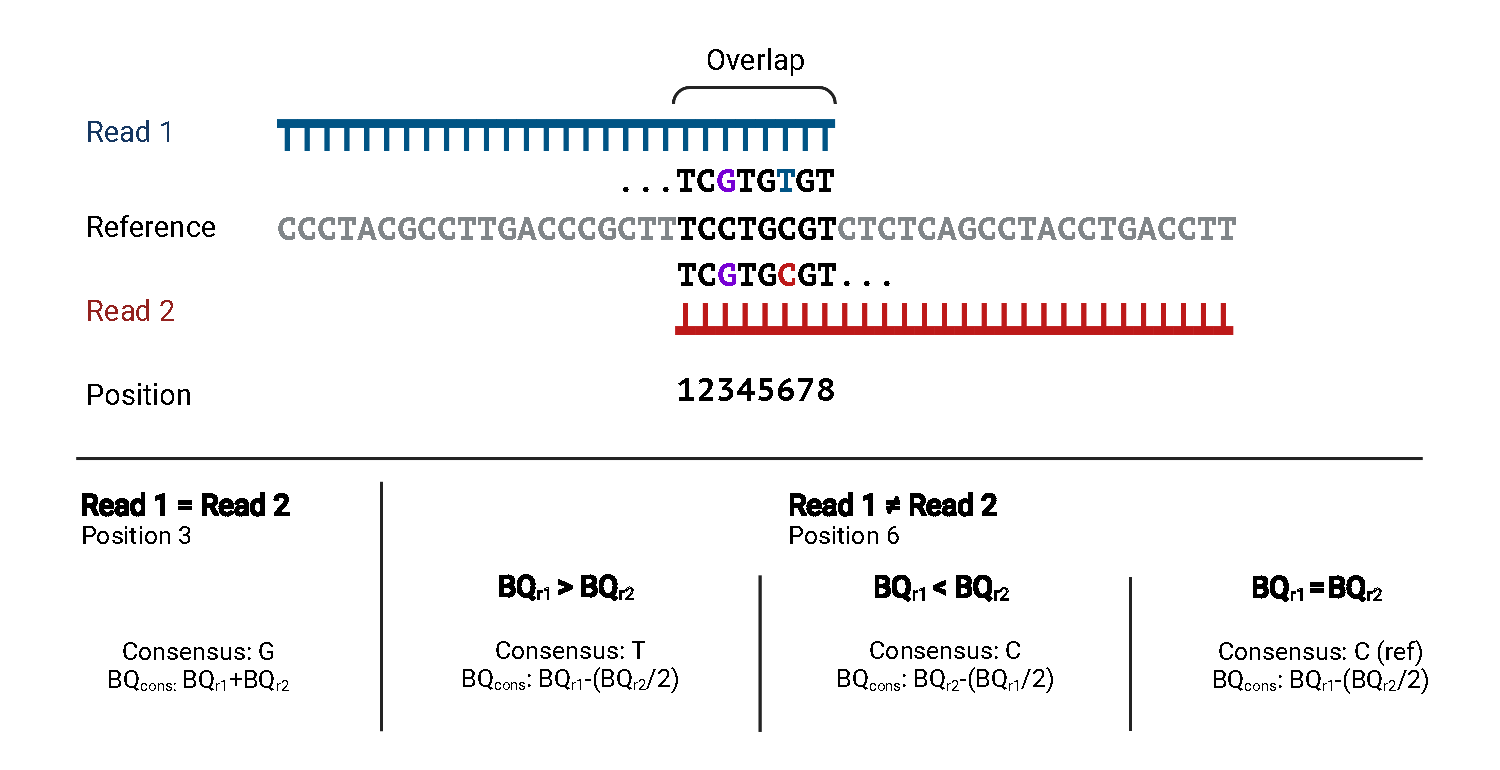
\includegraphics[width=.99\linewidth]{Figures/ConsensusMethodMisMatchFinder.pdf}
\caption[Schematic of consensus computation method for overlapping reads]{Schematic of consensus computation method for overlapping reads in MisMatchFinder; Read 1 and Read 2 depcit two overlapping paired end reads aligned to the reference sequence; Positions in the overlap are numbered for later referral; Read positions agreeing with the reference are coloured black, positions differeing from the reference but agreeing in both reads are coloured purple (position 3) and differences between reads are coloured in the respective read colours (blue and red, position 6); Calculation for the resulting base quality (BQ$_{cons}$ for each possibility is shown as formulas)}\label{fig:mmf-consensus}
\end{figure}


\section{Simulated data - the testing paradise}
\label{mmf-sec:simulated data}
Just like in \autoref{ch:variantcalling}, the novelty of the approach leads to the issue of no gold standard dataset, with which to evaluate the performance of a new method. While there are low coverage WGS datasets of cancer patients, none of them have validated signatures associated with them. So again simulated data is the optimal starting point to allow both optimisation of parameters as well as granular detection of artefacts which can originate from any step starting from sequencing over mapping to the signature deconvolution. 

\subsection{Sequencing errors - there is always a cleaner data}
\label{mmf-sec:cleanSim}
To judge the ability of our approach to filter out sequencing errors, we first simulated ``clean`` sequencing reads with neither germline or somatic variants with the ART simulation suite \cite{Huang2011}. As current estimates of Illumina sequencing is in the range of 1 in 666 to 1 in 1149 \cite{Stoler2021} which is significantly higher than even the highest tumour mutational burdens of  cancers (melanoma: 1 in 5k; tobacco smoking lung cancer: 1 in 100k) it is very important to be able to eliminate as much of the  background noise of sequencing errors as possible.

\begin{figure}[!ht]
\centering
\includegraphics[width=.99\linewidth]{Figures/mismatchrateCleanSequencing.pdf}
\caption[Mismatchrate of different filtering methods]{Mismatchrate of different filtering methods on sequencing data simulated with ART\cite{Huang2011} for both 10x and 3x coverage; Mismatches correspond to simulated sequencing errors; all: no filters, overlap: only use the overlapping parts of paired end reads with consensus building \protect\autoref{mmf-sec:consensus}, strict OL: overlap but reads \emph{must} agree, high BQ strict OL: strict OL with high BQ in both variants;}\label{fig:mmf-mismatchrate}
\end{figure}

By only using high base quality mismatches, where both reads agree on the mismatch 99.98\% of all sequencing errors can be eliminated and only 1 in 10M bases will be wrongly counted as a variant (\autoref{fig:mmf-mismatchrate}). This false discovery rate is multiple orders of magnitude lower than before and in a similar range to normal mutationally driven cancers tumour mutational burden \todo[color=red]{add citation}.

\todo[inline]{write about the germline filtering}